% Chapter 1

\chapter{Introducción} % Main chapter title

\label{introduction} % For referencing the chapter elsewhere, use \ref{Chapter1} 

%----------------------------------------------------------------------------------------

% Define some commands to keep the formatting separated from the content 
\newcommand{\keyword}[1]{\textbf{#1}}
\newcommand{\tabhead}[1]{\textbf{#1}}
\newcommand{\code}[1]{\texttt{#1}}
\newcommand{\file}[1]{\texttt{\bfseries#1}}
\newcommand{\option}[1]{\texttt{\itshape#1}}

%----------------------------------------------------------------------------------------


El origen de este trabajo iba a ser el estudio del modelo de crecimiento de galaxias bajo la influencia por una naturaleza \textit{warm dark matter} (WDM), en contraposición al modelo estandar asociado a la \textit{cold dark matter} (CDM). La finalidad era el estudio de la simulaciones de de WDM pero debido al escaso cat\'alogo de estas simulaciones y el estatus de este trabajo se opt\'o por otro enfoque. Dicho enfoque pas\'o desde una perspectiva enfocada a las simulaciones num\'ericas a un visi\'on m\'as te\'orica con la esperanza de poder ser traducida en un fut\'uro a una visi\'on m\'as pr\'actica.\\

El objeto de este trabajo es el \textit{Impossible Early Galaxy Problem} (IEGP) definido por primera vez en el paper \cite{steinhardt2016impossibly} c\'omo la discordancia encontrada en ese mismo paper sobre los datos deducidos de las observaciones de los campos CANDELS, SPLASH y CFHLS sobre la masa de los halos entre los redshift $4<z<7$ y los esperados por el modelo est\'andar. En dichas observaciones se encuentran un gran n\'umero de halos m\'uy masivos que quedar\'ian muy por encima de lo esperado por el modelo cosmol\'ogico $\Lambda$CMD y el modelo jer\'arquico de crecimiento gal\'actico.

\begin{figure}
	\begin{center}
		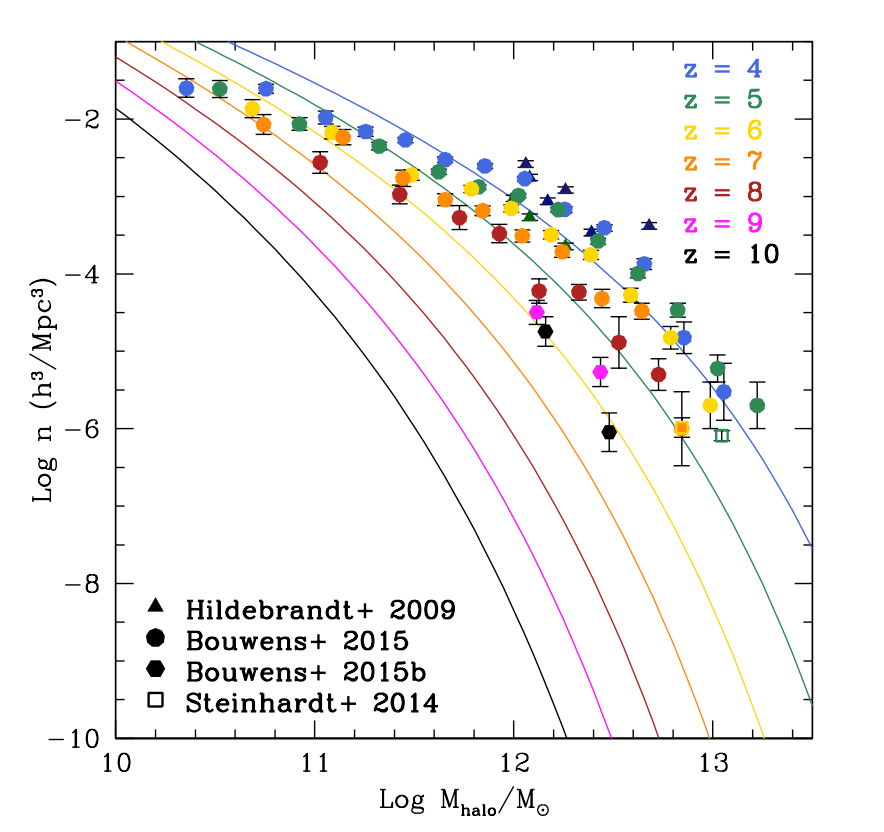
\includegraphics[scale=0.5]{Figures/steindhart_fig1}
		\caption{\label{fig:stein16_f1} Figura que representa la funci\'on de masa de halo. En l\'inea continua se muestra la predicci\'on te\'orica sacada de HMFCalc \citep{murray2013hmfcalc} y \cite{sheth2001ellipsoidal} mientr\'as que los marcadores muestran los valores obtenidos a trav\'es de las observaciones estudiadas en \cite{hildebrandt2009cars}, \cite{speagle2014highly} y \cite{bower2006breaking}.}
	\end{center}
\end{figure}

En esta pequeña sección discutiremos los principales puntos del paper de \cite{steinhardt2016impossibly}, las explicaciones y problemas dadas en él y por último estudiaremos como las nuevos valores obtenidos de \cite{behroozi2019universemachine} pueden contribuir a solucionar o agravar las discrepancias observadas. En las siguientes secciones trataremos el IEGP desde tres frentes distintos: el error de las observaciones, la naturaleza de la materia oscura y el modelo cosmológico considerado. Desde estas tres patas se intentará dar los ingredientes necesarios para las observaciones y la teoría vuelvan a poder encontrarse en armonía.


\section{The Impossible Early Galaxy Problem}